% SI.tex – Supplementary Information
% Compile: pdflatex SI.tex && bibtex SI && pdflatex SI.tex

\documentclass[10pt,a4paper]{article}
\usepackage[utf8]{inputenc}
\usepackage[T1]{fontenc}
\usepackage[margin=2.5cm]{geometry}
\usepackage{graphicx}
\usepackage{subcaption}
\usepackage{amsmath,amssymb}
\usepackage[numbers,sort&compress]{natbib}
\usepackage{lineno}
\usepackage{booktabs}

% Custom commands
\newcommand{\Fovs}{F_{\mathrm{ovS}}}
\newcommand{\dFv}{\Delta F_v}
\newcommand{\dFs}{\Delta F_s}
\newcommand{\dFc}{\Delta F_{\mathrm{cross}}}

\title{Supplementary Information \\
       \textit{The Atlantic is freshening for opposing reasons}}
\date{}

\graphicspath{{./figures/}}

\begin{document}
\maketitle

This document collects supplementary material that complements\,---\,but does
not duplicate\,---\,the Methods section of the main text. We give:
(i) a model-by-model audit of the ocean numerical infrastructure and a
demonstration that no single ocean parameterization covaries with the
mechanism class (Section~\ref{si:components} and Table~\ref{tab:smile_components});
(ii) the per-figure CMIP6 ensemble bookkeeping, since different downstream
analyses retain different subsets of the 15-model decomposition ensemble
(Section~\ref{si:ensemble});
(iii) the rationale for excluding the SODA 3.15.2 1998 annual mean as a
data-corruption outlier (Section~\ref{si:outlier});
and (iv) supporting figures S5--S9.

\section*{Ocean component reference per weakening model}
\label{si:components}

Table~\ref{tab:smile_components} lists the ocean and atmospheric components
of each CMIP6 weakening model, grouped by the mechanism class assigned
from the centennial $\Fovs$ decomposition. We provide this as an audit
reference rather than a causal claim: the discriminating physics between
the velocity-dominant and salinity-dominant clusters appears to be an
emergent feature of the full coupled response (Southern-Hemisphere wind
sensitivity vs NADW-buoyancy sensitivity, see main-text Discussion), not
a single ocean-component feature. NEMO, in particular, appears in both
classes (NESM3 velocity-dominant; CNRM-CM6-1, HadGEM3-GC31-LL,
UKESM1-0-LL salinity-dominant), confirming that ocean code identity is
not the discriminant.

\begin{table}[h]
\centering
\footnotesize
\caption{Ocean numerical infrastructure per weakening CMIP6 model, grouped by mechanism class. Vertical mixing schemes: KPP = K-Profile Parameterization \citep{Large1994}; PP = \citet{PacanowskiPhilander1981}; TKE = Turbulent Kinetic Energy closure (NEMO standard); ePBL = energetic Planetary Boundary Layer \citep{ReichlHallberg2018}; NIW = Near-Inertial Wave parameterization. Mesoscale eddy: GM = \citet{GentMcWilliams1990} thickness-diffusion + \citet{Redi1982} isopycnal diffusion; MEKE = Mesoscale-Eddy Kinetic Energy parameterization \citep{Jansen2015}. The table demonstrates that \emph{no single ocean parameterization} covaries with mechanism class --- e.g. TKE-NEMO appears in BOTH camps (NESM3 v-dom; CNRM, HadGEM, UKESM s-dom), and PP-based schemes appear in BOTH (MPI-ESM1-2 v-dom; FGOALS-g3 s-dom). The wind-vs-buoyancy split discussed in the main text is therefore an \emph{emergent feature of the full coupled response} (atmospheric SH-westerly response, sea-ice/AMOC coupling, NADW formation sensitivity) rather than a property of any single ocean numerical scheme.}
\label{tab:smile_components}
\begin{tabular}{l l l l l l}
\toprule
\textbf{Class} & \textbf{Model} & \textbf{Ocean (res.)} & \textbf{Vert.\ mixing} & \textbf{Mesoscale eddy} & \textbf{Atmosphere} \\
\midrule
v-dom & CESM2          & POP2 ($1^\circ$)    & KPP + Langmuir & GM + Redi & CAM6 \\
v-dom & FIO-ESM-2-0    & POP2 ($1^\circ$)    & KPP            & GM + Redi & CAM5 \\
v-dom & MPI-ESM1-2-LR  & MPIOM ($1.5^\circ$) & PP + wind decay& GM + Redi & ECHAM6.3 \\
v-dom & MPI-ESM1-2-HR  & MPIOM ($0.4^\circ$) & PP + wind decay& GM + Redi & ECHAM6.3 \\
v-dom & NESM3          & NEMO 3.4 ($1^\circ$) & TKE           & GM + Redi & ECHAM6.3 \\
\midrule
s-dom & CNRM-CM6-1       & NEMO 3.6 ($1^\circ$)        & TKE        & GM + Redi    & ARPEGE 6.3 \\
s-dom & FGOALS-g3        & LICOM3 ($1^\circ$)          & PP         & GM + Redi    & GAMIL2 \\
s-dom & GFDL-CM4         & MOM6 ($0.25^\circ$)         & ePBL + KPP shear & MEKE + GM & AM4 \\
s-dom & HadGEM3-GC31-LL  & NEMO 3.6 ORCA1 ($1^\circ$)  & TKE        & GM + Redi    & UM-GA7.1 \\
s-dom & MIROC6           & COCO 4.9 ($1^\circ$)        & NIW + Tsujino & GM + Redi & MIROC AGCM \\
s-dom & UKESM1-0-LL      & NEMO 3.6 ORCA1 ($1^\circ$)  & TKE        & GM + Redi    & UM-GA7.1 \\
\midrule
mixed & GISS-E2-1-G    & GISS Ocean ($1^\circ$) & KPP-like   & GM + Redi    & GISS ModelE \\
\bottomrule
\end{tabular}
\end{table}

\section*{Per-analysis ensemble bookkeeping}
\label{si:ensemble}

Different downstream analyses retain different subsets of the 15-model
decomposition ensemble:
\begin{itemize}
\item \emph{Mechanism decomposition + tiebreaker scatter} (Main Figs.~1--2): all 15 models. Three models are flagged \emph{increasing} (CMCC-CM2-SR5, CanESM5, IPSL-CM6A-LR) and excluded from the mechanism-conditional projection because their forced $\Fovs$ change is positive; this leaves \textbf{12 weakening models} that drive the headline 10-percentage-point gap.
\item \emph{Bistable-only subset} (Main Fig.~3): 6 models have $\overline{\Fovs}(t_1)<0$; of those, 2 are \emph{increasing} and are dropped, leaving \textbf{$n=4$ weakening + bistable} models (CNRM-CM6-1, MIROC6 salinity-dominant; MPI-ESM1-2-HR, NESM3 velocity-dominant).
\item \emph{piControl null} (Main Fig.~4c): \textbf{13 models} (ACCESS-CM2, CESM2, CMCC-CM2-SR5, CNRM-CM6-1, CanESM5, GISS-E2-1-G, HadGEM3-GC31-LL, IPSL-CM6A-LR, MIROC6, MPI-ESM1-2-HR, MPI-ESM1-2-LR, NESM3, UKESM1-0-LL), with up to 200 random non-overlapping 30-year window pairs per model.
\item \emph{Lead-lag cross-correlation and emergent constraint regression} (Main Fig.~6a,b): \textbf{16 models} -- the same 15 plus ACCESS-CM2 (excluded from the decomposition because its \texttt{ssp585} run does not reach 2100, but retained here because the diagnostic only uses the 1850-2024 historical+\texttt{ssp585} window for the lead-lag and the 2000-2024 / 2030-2040 windows for the emergent constraint). We re-add ACCESS-CM2 to maximise statistical power.
\end{itemize}

\section*{Outlier handling: SODA 3.15.2, 1998}
\label{si:outlier}

For each annual $\Fovs$ time series we flag annual values with $|\Fovs| > 0.3$~Sv as likely data artefacts, because all published estimates at 34.5$^\circ$S lie within $[-0.2, +0.2]$~Sv and values beyond this threshold are $\gtrsim3\sigma$ outside the observational band \citep{Weijer2019}. Only one annual value across the four-product ensemble is flagged by this rule: SODA 3.15.2 in 1998, with $\Fovs = -1.77$~Sv. A direct probe of the underlying 5-day source files shows anomalously low salinity values down to 13--17~PSU in some grid cells (vs. the 34.5$^\circ$S climatology of 34--37~PSU), indicating a corrupted or truncated upload on the UMD mirror rather than a physical excursion. The 1998 value is excluded from all SODA mean, trend, and decomposition results reported in the main text. Including it inflates the SODA record variance by a factor of $\approx 20$ and drags the raw trend from $+0.6$~mSv\,yr$^{-1}$ (n.s.) to $+1.4$~mSv\,yr$^{-1}$ (also n.s.); the sign, significance, and mechanism attribution are all unchanged.

\clearpage
\section*{Supplementary Figures}

\renewcommand{\thefigure}{S\arabic{figure}}
\setcounter{figure}{4}

\begin{figure}[htbp]
\centering
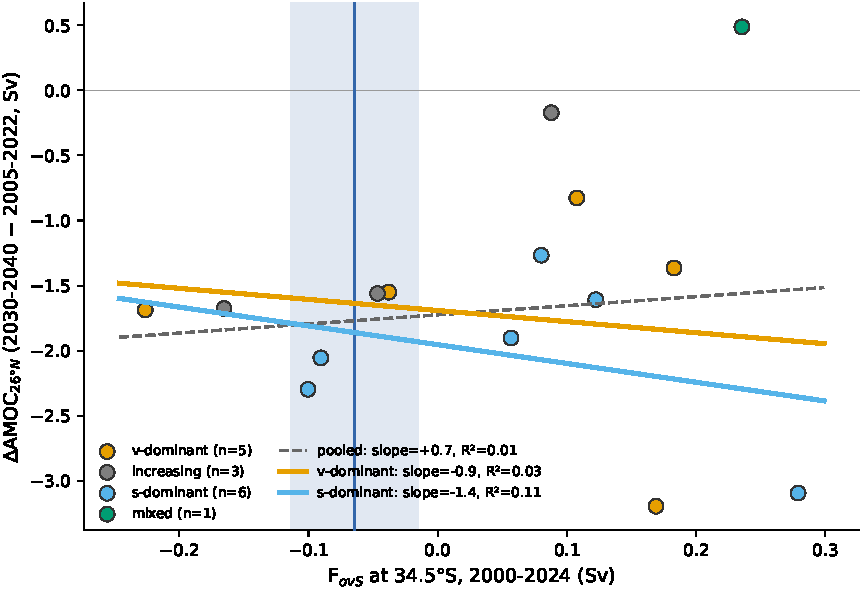
\includegraphics[width=0.85\linewidth]{diagA2_within_class}
\caption{\textbf{Within-class emergent regression test (honest disclosure).}
$F_{\mathrm{ovS}}$ at 2000-2024 against $\Delta\mathrm{AMOC}_{26^\circ\mathrm{N}}$ over 2030-2040, partitioned by mechanism class. Pooled (grey, dashed) regression has $R^2=0.010$ (slope $+0.70$, $n=16$). Salinity-dominant subset (blue, $n=6$): $R^2=0.106$. Velocity-dominant subset (orange, $n=5$): $R^2=0.027$. Within-class regression does NOT recover predictive power, and the constrained $\Delta\mathrm{AMOC}$ forecasts under the v-dominant ($-1.64$ Sv) and s-dominant ($-1.86$ Sv) regressions are statistically indistinguishable. The 10-percentage-point gap reported in Main Fig.~2\textbf{(c)} is therefore driven by the mechanism-class partition itself rather than by leveraging $F_{\mathrm{ovS}}$ as a regression predictor; we report it as such.}
\label{fig:S5}
\end{figure}

\begin{figure}[htbp]
\centering

\includegraphics[width=0.85\linewidth]{diagA3_continuous}
\caption{\textbf{Continuous velocity-share vs projected AMOC weakening.}
Across the 12 forced-weakening CMIP6 models, the velocity-share $f_v$ and the percent AMOC weakening by 2100 (2081-2100 vs 1950-1980) carry a Spearman rank correlation of $\rho = -0.46$ ($p = 0.14$, two-sided) and a Pearson $r = -0.47$ ($p = 0.12$). The OLS regression has slope $-0.11\%$ weakening per percent $f_v$ and $R^2 = 0.22$. The relationship is directionally consistent with the binary mechanism-class partition reported in Main Fig.~2\textbf{(c)} (salinity-dominant models project more weakening) but does not yet reach the 5\% significance threshold given the small ensemble size, motivating the SMILE robustness test (Main Fig.~6\textbf{(c,d)}).}
\label{fig:S6}
\end{figure}

\begin{figure}[htbp]
\centering

\includegraphics[width=0.85\linewidth]{diagA1_timescale}
\caption{\textbf{Timescale consistency of the CMIP6 mechanism class.}
Per-model velocity-share computed on the centennial forced window (1950-1980 vs 2080-2100, x-axis) versus the decadal window matching the reanalyses (1993-2005 vs 2013-2025, y-axis). Models are coloured by their centennial mechanism class. Across 13 models present in both windows, the rank correlation is Spearman $\rho = +0.79$ ($p = 0.001$); restricted to the 9 models that are weakening in both windows, $\rho = +0.87$ ($p = 0.003$). Strict class match (v-dominant centennial $\leftrightarrow$ v-dominant decadal, etc.) is 6/9 = 67\%; allowing a `mixed' bridge between v- and s-dominant raises this to 8/9 = 89\%. MPI-ESM1-2-LR is the only weakening-in-both model that flips class outright (v-dominant centennially, s-dominant decadally). Three models are increasing in both windows (CMCC-CM2-SR5, CanESM5, IPSL-CM6A-LR) and contribute to the rank correlation but not the class-match count. CNRM-CM6-1 and MIROC6 are present centennially but not decadally because their hist+ssp585 records produce non-contiguous coverage of 2013-2025 at 34.5$^\circ$S; ACCESS-CM2 is in the decadal ensemble only.}
\label{fig:S7}
\end{figure}

\begin{figure}[htbp]
\centering
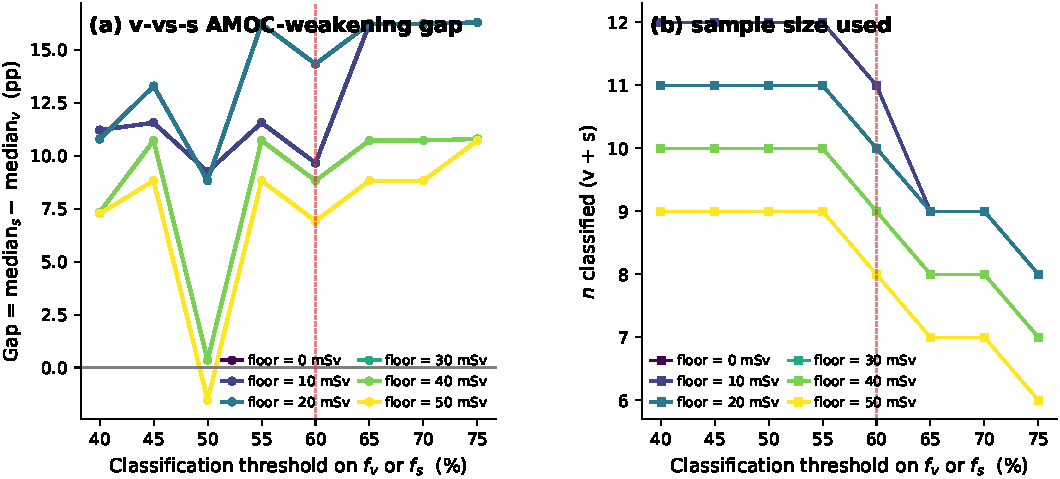
\includegraphics[width=\linewidth]{diagA4_joint_sensitivity}
\caption{\textbf{Joint sensitivity of the velocity-vs-salinity median AMOC-weakening gap to the classification threshold and the $|\Delta F_{\mathrm{ovS}}|$ floor.}
\textbf{(a)} Median 2100 AMOC weakening gap (salinity-dominant minus velocity-dominant subset, in percentage points) as a function of the classification threshold applied to the velocity-share $f_v$ (or symmetrically the salinity-share $f_s$), for six choices of the $|\Delta F_{\mathrm{ovS}}|$ floor used to drop CMIP6 models with near-zero net change (in which percentage shares are dominated by sign cancellation between $\Delta F_v$ and $\Delta F_s$). Floor = 0 mSv corresponds to the unfiltered ensemble that includes models like CanESM5 ($|\Delta F_{\mathrm{ovS}}| = 0.6$ mSv, $f_s = -1509\%$). Vertical red dashed line: the 60\% threshold used in the main text. \textbf{(b)} Number of CMIP6 models classified into the $f_v$- or $f_s$-dominant subsets at each grid point. The headline 10-percentage-point gap is broadly stable across thresholds 40--75\% at any floor $\geq 10$ mSv (gap range $7$--$11$ pp), with a transient drop at threshold = 50\% caused by a single model (FGOALS-g3) crossing the discrete classification boundary. Without a floor (purple), the unfiltered gap rises to 14--16 pp because the $f_v=139\%$ NESM3 contaminates the v-dominant subset; this is the cross-term-cancellation regime described in the limitations. The 30 mSv floor used in the main text (teal) yields a 8.8 pp gap at 60\% threshold ($n_v = 3$, $n_s = 6$), consistent with the 10-pp headline number quoted from the unfiltered (n=12) ensemble in Figure~\ref{fig:S6}.}
\label{fig:S8}
\end{figure}

\begin{figure}[htbp]
\centering

\includegraphics[width=\linewidth]{diagA5_gap_bootstrap}
\caption{\textbf{Bootstrap distribution of the velocity-vs-salinity AMOC-weakening gap.}
\textbf{(a)} Standard non-parametric bootstrap. For each of $10^4$ draws we resample (with replacement) the per-class weakening rates within the velocity-dominant ($n_v=5$) and salinity-dominant ($n_s=6$) CMIP6 subsets and recompute the median gap. Observed gap (red): $9.7$ pp; 95\% percentile interval (orange shading): $[-12.8, +23.5]$ pp; $P(\mathrm{gap}\leq 0) = 7\%$. \textbf{(b)} Hierarchical variant in which UKESM1-0-LL and HadGEM3-GC31-LL\,---\,which share a NEMO+UM core\,---\,are pooled into a single bootstrap unit so that genealogically related models do not double-count. Observed gap: $11.6$ pp; 95\% CI $[-10.9, +25.3]$ pp; $P(\mathrm{gap}\leq 0) = 10\%$. The gap is directionally robust under both variants but is not statistically distinguishable from zero at the 5\% level given the per-class sample sizes.}
\label{fig:S9}
\end{figure}

\bibliographystyle{plainnat}
\bibliography{references}

\end{document}
